\documentclass[dvipdfmx]{jsarticle}
\usepackage{MyPackage}
\usepackage{tikz}
\title{組み合わせ計算の例題}
\author{}
\date{}

\begin{document}
\maketitle
    この資料の内容は以下の4つの例題に対する解答である.解答を見る前に各自で解いてみることを進める.
    \begin{enumerate}
        \item 1から6までの番号が振られた6つの球を箱A,B,Cに自由に入れるときの組み合わせの総数.
        \item 1から6までの番号が振られた6つの球を3の箱に自由に入れるときの組み合わせの総数.ただし,箱は同じものが3つであり,空となる箱が生まれても良い.
        \item 6つの球を箱A,B,Cに自由に入れるときの組み合わせの総数.ただし,球はすべて同じものである.
        \item 6つの球を3つの箱に自由に入れるときの組み合わせの総数.ただし,球も箱もそれぞれすべて同じものである.
    \end{enumerate}

    \section{問1}
    1番目の問題は区別あるもの(番号付きの球)を区別のある選択肢(箱A,B,C)へ分ける問題である.分けるものは1から6までの球であるが,それらがすべて独立して3つの選択肢(A,B,C)を持っている.したがって答えは
    \[
    3\times 3\times \cdots \times 3 = 3^6
    \]
    と計算される.

    分けるもの(球),分ける先(箱)の両方に区別がある場合は,分けるもの(球)の1つ1つに対して選択肢を考え,最終的に掛け算によって全体の事象を考える.これは系統樹を書くことで説明できる話だ.

    \section{問2}
    2番目の問題では,区別があるもの(番号付きの球)を区別のない選択肢(3つの箱)へ分ける問題である.普通に数え上げる方法では,まず答えにたどり着かない難問になっている.

    解法の鍵は問1の結果を利用することにある.例えば次の3つの分配は問1の状態では区別されたが,本問では箱の区別がないので同じものと考えられる.
    \[
    A\{1,2\},\qquad B\{3,4\},\qquad C\{5,6\}
    \]

    区別をなくすというのは,
    \[
    \{1,2\},\qquad \{3,4\},\qquad \{5,6\}
    \]
    という3つのグループの分かれ方が問1では \(3!\)だけ数えられていたところを1つと考えることである.つまりは, \(3!\)で割ることが必要なのだ.しかし,それだけでは正確ではない.

    \[
    \{1,2,3,4,5,6\},\qquad \{\},\qquad\{\}
    \]

    と分かれた場合は問1において3通り,本問では1通りとなり, \(3!\)で割ると減らしすぎとなってしまう.以上のことから,本問の計算は次の2点を抑えることでできる.
    \begin{itemize}
        \item 問1の \(3^6\)のうち, \(3^6-3\)は \(3!=6\)で割る.
        \item 問1の \(3^6\)のうち,3は3で割る.
    \end{itemize}
    これらの和をとることで
    \[
    \frac{3^6-3}{3!}+\frac{3}{3} = \frac{3^5-1}{2} +1 =122
    \]
    と計算される.

    要は問1で数えすぎた分を適切に減らしてゆくという問題になっている.空箱が0または1つの場合は箱に入った球の番号から,3つのグループをすべて区別できる.そのため \(3!\)倍数えすぎているとわかる.対して,空箱が2つある場合は空箱2つの区別がつかない.そのため3倍数えすぎているとわかる.あとは数えすぎた分を割ればよい.

    \section{問3}
    3番目の問題では,区別のないもの(6つの球)を区別のある選択肢(箱A,B,C)へ分ける問題である.

    3つの解法がある.それぞれマスターしよう.
    \subsection{代数的な解法}
    箱A,B,Cに入る球の個数を \(a,b,c\)とする.すると次の方程式が立てられる.
    \[
    a+b+c=6,\quad a,b,c\geq 0
    \]
    この方程式の整数解 \((a,b,c)\)を計算すればいい.

    \(a=0\)のとき, \(b+c=6\)である.ここから,
    \[
    (b,c)=(0,6),\ (1,5),\ (2,4),\ (3,3),\ (4,2),\ (1,5),\ (0,6)
    \]
    となる.解の個数は7個である.これを同様に \(a=1,2,\cdots,6\)まで計算すると,それぞれ解の個数が6個,5個,,,1個となる.解の個数を合計することで組み合わせの数は28と計算される.

    この解法では組み合わせの数を方程式の解の個数に置き換えて計算している.まず思いついてほしい解法である.

    \subsection{個数の分配}
    この問題では分けるものに区別がなく,分ける先に区別がある.このような場合は分けるものである球ではなく,分ける先である箱に注目する必要がある.

    このような考え方は個数の分配を考えるものであり,最初の解法はそれを方程式で実現したものだ.ここでは個数の分配をより原始的に考える.6個の球を3つに分けることを考えると,それは2つの仕切りを置くことといえる.仕切りを置いたら,必ず左をAに,真ん中をBに,右をCにすると決めておくことで分配は完了する(図\ref{tikz_kosuu_bunpai}).

    \begin{figure}[htbp]\centering
        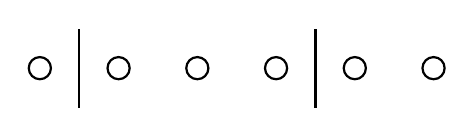
\begin{tikzpicture}\large
            \foreach \x in {0,...,5}{
            \draw[thick] (\x,0) circle (4pt);
            }
            \draw[thick](0.5,-0.5)--(0.5,0.5);
            \draw[thick](3.5,-0.5)--(3.5,0.5);
        \end{tikzpicture}
        \caption{個数の分配}
        \label{tikz_kosuu_bunpai}
    \end{figure}

    この考え方だと,6つの球と2つの仕切りの順列となるので次の式で組み合わせの個数が計算される.
    \[
    \frac{8!}{6!2!} = {}_8 \mathrm{C}_2 = 28
    \]

    \subsection{重複順列}
    最後は理解ができれば最も簡単な解法だ.本問はA,B,Cという箱の選択肢を被ること(重複)を認めて,6つ選択するものである.それはすなわち,重複順列である.組み合わせは
    \[
    {}_3 \mathrm{H}_6
    \]
    と計算される.
    \[
    {}_n\mathrm{H}_r = {}_{n+r-1}\mathrm{C}_r
    \]
    という公式があるので,計算する.
    \[
    {}_3 \mathrm{H}_6={}_8 \mathrm{C}_6 = 28
    \]

    \vspace{3eX}
    3つの解法をすべてマスターしよう.

    \section{問4}
    4番目の問題では区別のないもの(6つの球)を区別のない選択肢(3つの箱)へ分ける問題である.このような問題では単純に足せば6になる3つの数の組を探すことになる.(1,2,3)と(3,2,1)は同じものとして考えるので,問3の代数的な解法をもう少しだけ改良することで解く.

    \[
    a+b+c=6,\qquad 0\leq a\leq b\leq c
    \]
    この方程式の解の個数が組み合わせの個数になる.先と違うのは \((a,b,c)\)に大小関係があることだ.これによって入れ替えた解を省くことができる.

    \(a=0\)のとき, \(b+c=6,0\leq b\leq c\)であるから
    \[
    (b,c) = (0,6),\ (1,5),\ (2,4),\ (3,3)
    \]
    の4つが解となる.同様に \(a=1,2\)のときで計算すると解の個数はそれぞれ2個と1個得られる.すべての解の個数は7個となり,これが組み合わせの個数となる.


    \section*{まとめ}
    分けるもの・分ける先の区別の有無によって,組み合わせの個数の計算方法は全く違う.したがって,組み合わせの個数を計算するときは必ず分けるもの・分ける先を明確にして区別の有無を確認しなければならない.







\end{document}
